\documentclass[xetex,mathserif,serif]{beamer}
\usepackage{polyglossia}
\setdefaultlanguage[babelshorthands=true]{russian}
\usepackage{minted}
\usepackage{tabu}
\usepackage{graphicx}

\useoutertheme{infolines}

\usepackage{fontspec}
\setmainfont{FreeSans}
\newfontfamily{\russianfonttt}{FreeSans}

\definecolor{links}{HTML}{2A1B81}
\hypersetup{colorlinks,linkcolor=,urlcolor=links}

\setbeamertemplate{blocks}[rounded][shadow=false]
\setbeamercolor*{block title alerted}{fg=red!50!black,bg=red!20}
\setbeamercolor*{block body alerted}{fg=black,bg=red!10}

\tabulinesep=0.8mm

\title{Классификация текстового контента}
\author{Александр Смирнов и Феодор Жилкин}
\date{17.05.2019г}

\begin{document}

	\frame{\titlepage}

	\begin{frame}
		\frametitle{Введение}
		\begin{figure}[h]
            \center{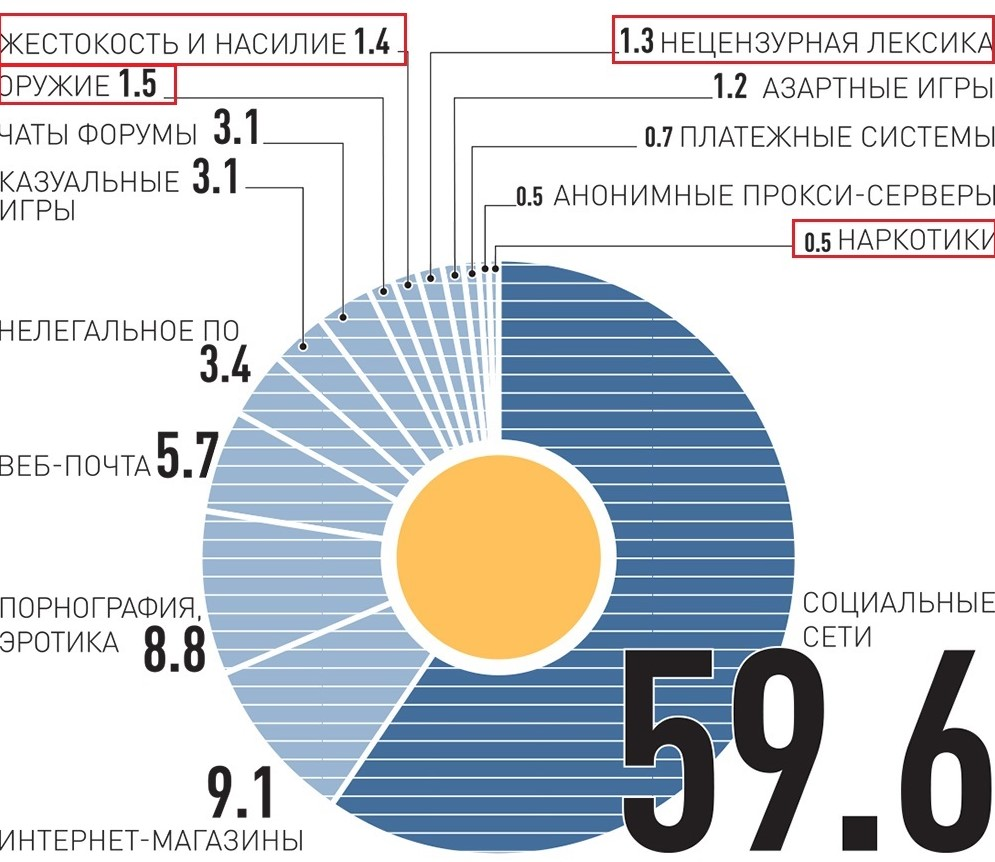
\includegraphics[scale=0.75]{images/children_statistics.jpg}}
            \caption{Что интересует детей в интернете}
            \label{fig:image}
        \end{figure}
	\end{frame}
	
	\begin{frame}
		\frametitle{Цели}
			\begin{itemize}
		 		\item Ограничить детей от взрослого текстового контента
				\item Получение опыта
    				\begin{itemize}
    			    	\item Нейросети
    			    	\item Python, Jupyter Notebook, JS
    			    	\item Майнинг датасета и составление csv-файла для загрузки на \url{https://www.kaggle.com}
    			    	\item Написание собственной Python-библиотеки
    			    	\item Написание расширения для Chrome
    			    	\item Написание Python-сервера для приёма запросов
    		    	\end{itemize}
			\end{itemize}
	\end{frame}
	
	\begin{frame}
		\frametitle{Задачи}
			\begin{itemize}
		 		\item Сделать расширение для Chrome
				\item Внести вклад в сообщество разработчиков
					\begin{itemize}
				    	\item Датасет на \url{https://www.kaggle.com}
				    	\item Python-библиотека
			    	\end{itemize}
			\end{itemize}
	\end{frame}	
	
	\begin{frame}
		\frametitle{Сравнение с аналогами}
			\begin{itemize}
				\item Ограничения на поиск
					\begin{itemize}
				    	\item Семейный поиск Яндекс
				    	\item Безопасный поиск Google
			    	\end{itemize}
			    \item Контентная фильтрация
					\begin{itemize}
				    	\item Traffic Inspector
				    	\item Интернет Цензор
			    	\end{itemize}
			\end{itemize}
	\end{frame}

	\begin{frame}
		\frametitle{Результаты}
		\begin{itemize}
			\item Расширение для Chrome
			\item Библиотека на \url{https://pypi.org/project/TalesParse/}
			\item Датасет на \url{https://www.kaggle.com/idoldev/adult-and-child-russian-tales-dataset-with-label}
		\end{itemize}
	\end{frame}
	
	\begin{frame}
		\frametitle{Результаты обучения}
	    	\begin{columns}[t]
                \column{.3\textwidth}
                    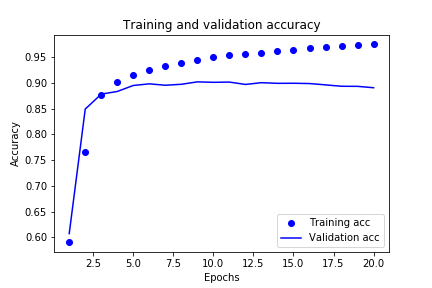
\includegraphics[scale=0.35]{images/acc.png}
                \column{.3\textwidth}
                    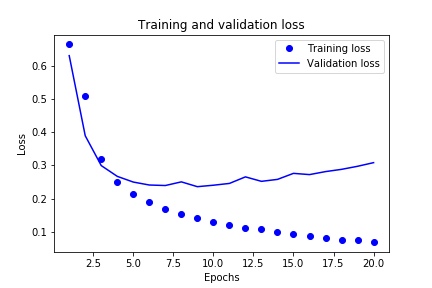
\includegraphics[scale=0.35]{images/loss.png}
                \column{.05\textwidth}
            \end{columns}
	\end{frame}		
	
	\begin{frame}
		\frametitle{Расширение для Chrome (1)}
		\begin{figure}[h]
            \center{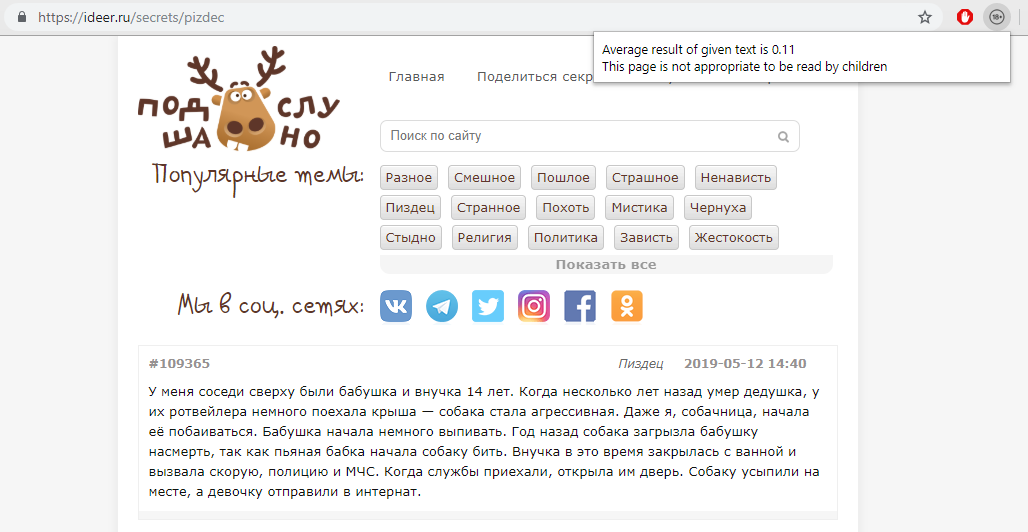
\includegraphics[scale=0.4]{images/bad_content_example.png}}
            \caption{Блокировка контента}
            \label{fig:image}
        \end{figure}
	\end{frame}	
	
	\begin{frame}
		\frametitle{Расширение для Chrome (2)}
		\begin{figure}[h]
            \center{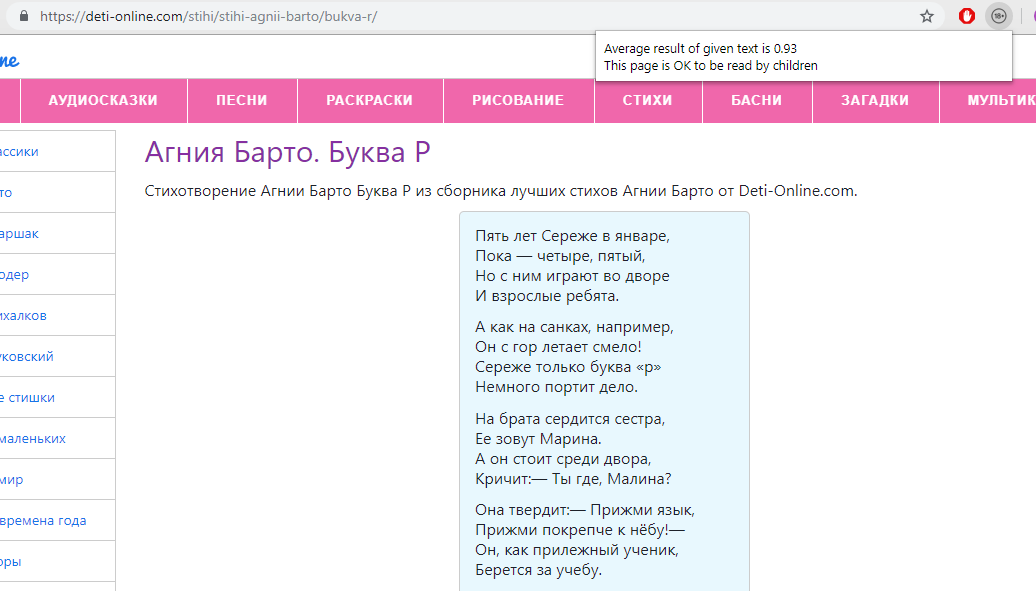
\includegraphics[scale=0.37]{images/good_content_example.png}}
            \caption{Допуск до контента}
            \label{fig:image}
        \end{figure}
	\end{frame}	
	
	\begin{frame}
		\frametitle{Библиотека на pypi}
		\begin{figure}[h]
            \center{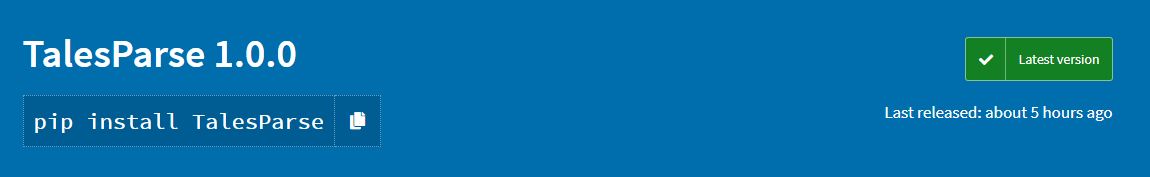
\includegraphics[scale=0.6]{images/library.png}}
            \caption{Библиотека}
            \label{fig:image}
        \end{figure}
	\end{frame}	
	
	\begin{frame}
		\frametitle{Датасет на kaggle}
		\begin{figure}[h]
            \center{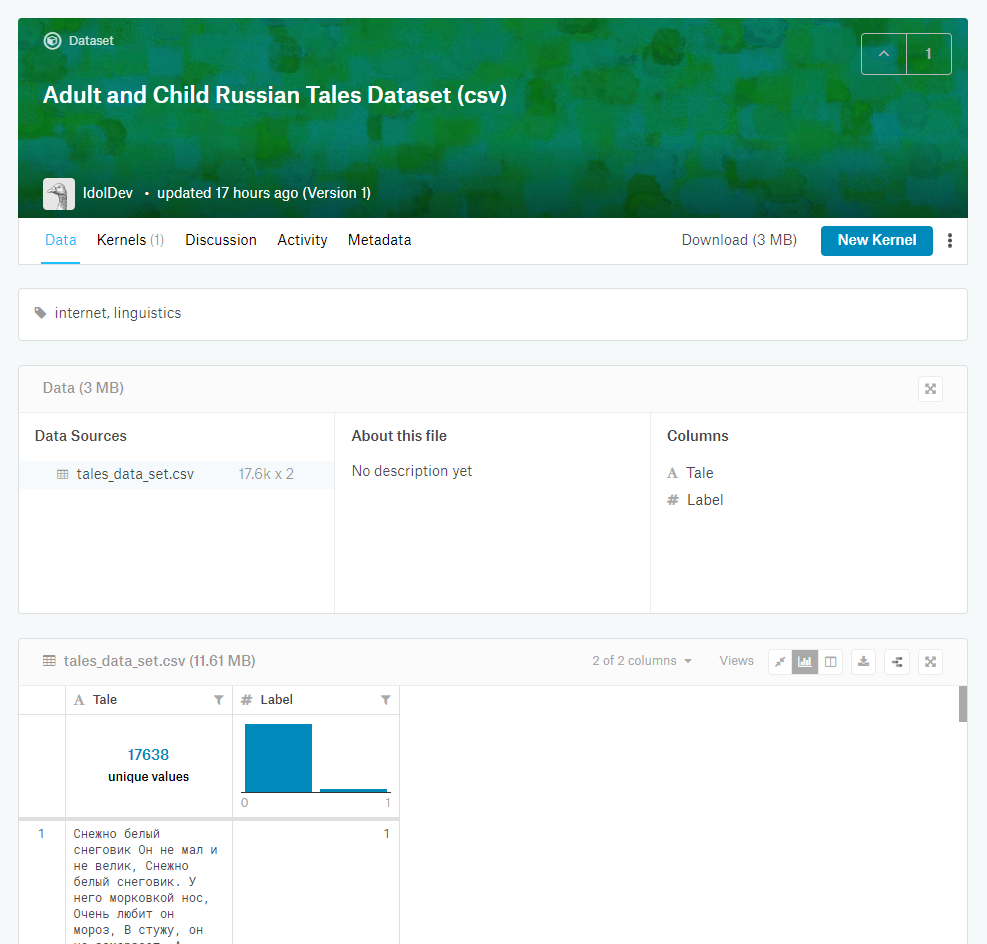
\includegraphics[scale=0.25]{images/kaggle.png}}
            \caption{Датасет}
            \label{fig:image}
        \end{figure}
	\end{frame}
	
	\begin{frame}
		\frametitle{Как это всё работает}
		\begin{figure}[h]
            \center{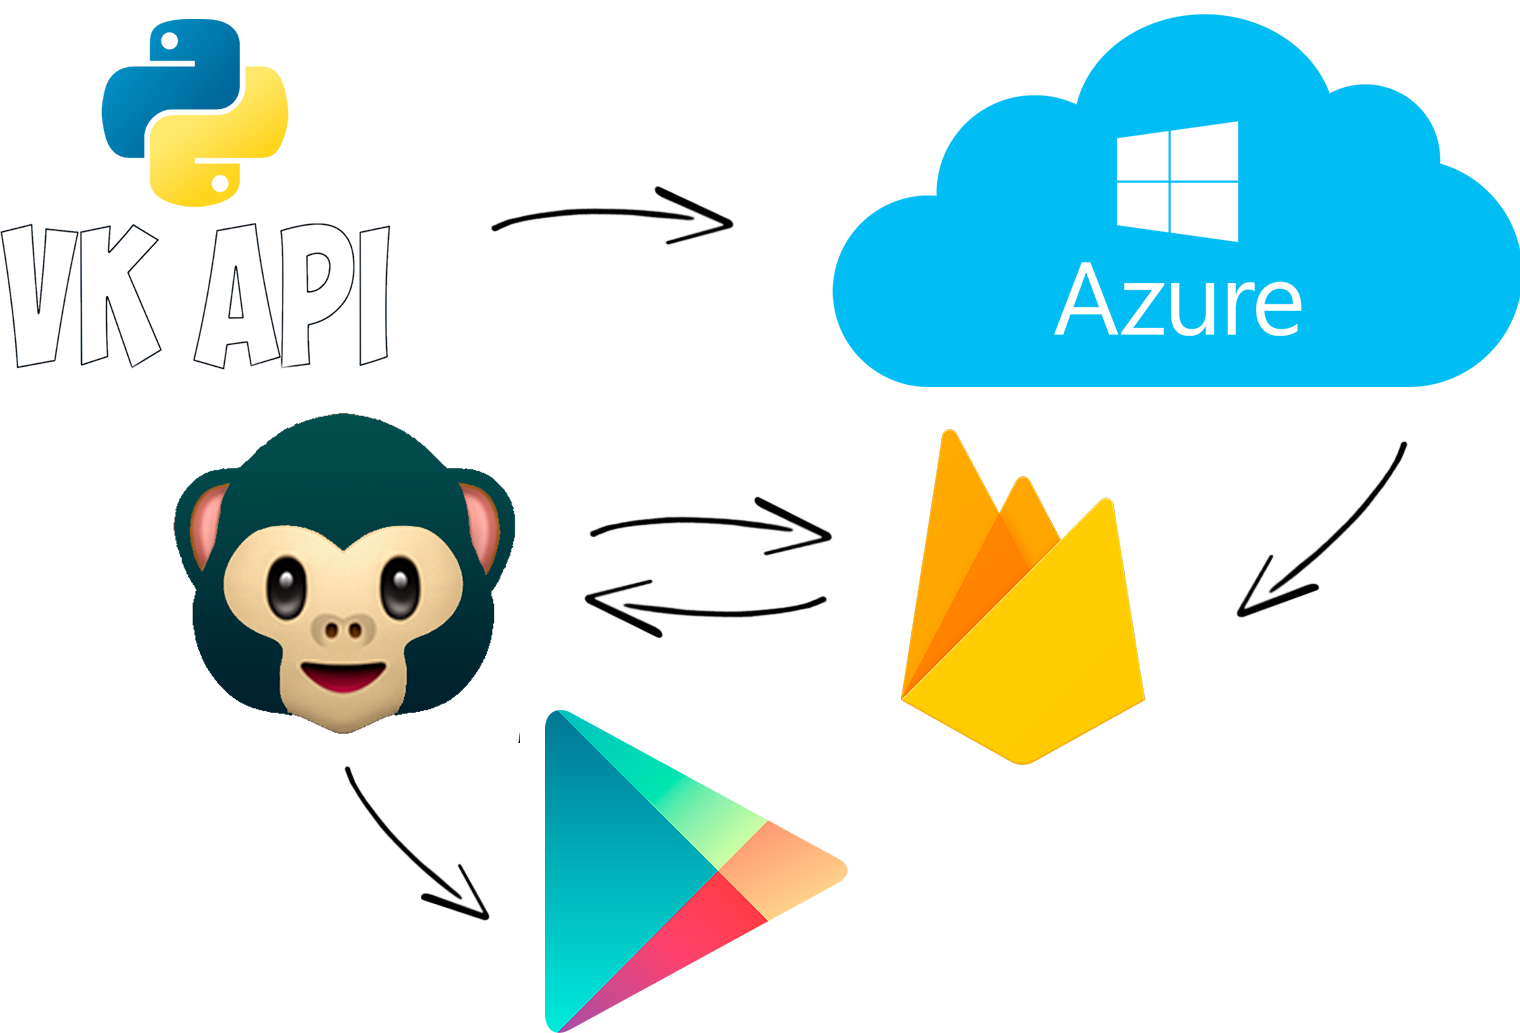
\includegraphics[scale=0.2]{images/scheme.png}}
            \caption{Схема проекта}
            \label{fig:image}
        \end{figure}
	\end{frame}	
	
	\begin{frame}
		\frametitle{Итоги}
		\begin{itemize}
			\item Феодор
			    \begin{itemize}
			    	\item Парсинг
			    	\item Python-библиотека
			    	\item Датасет
		        \end{itemize}
			\item Александр
			    \begin{itemize}
			    	\item Нейросеть
			    	\item Сервер
			    	\item Расширение
		        \end{itemize}
		\end{itemize}
	\end{frame}
	
	\begin{frame}
		\frametitle{Результаты}
		\begin{itemize}
			\item Проект – \url{https://github.com/SmirnovAlexander/PoemClassifier}
			\item Парсер – \url{https://github.com/Feodoros/Scraping_Tales}
			\item Библиотека – \url{https://pypi.org/project/TalesParse/}
			\item Датасет – \url{https://www.kaggle.com/idoldev/adult-and-child-russian-tales-dataset-with-label}
		\end{itemize}
	\end{frame}

\end{document}